\documentclass[11pt]{article}
% Some packages I commonly use.
\usepackage[english]{babel} \usepackage{graphicx} \usepackage{framed}
\usepackage[normalem]{ulem} \usepackage{amsmath} \usepackage{amsthm}
\usepackage{amssymb} \usepackage{multirow} \usepackage{multicol}
\usepackage{adjustbox} \usepackage{amsfonts} \usepackage{enumerate}
\usepackage[utf8]{inputenc} \usepackage[top=1 in,bottom=1in, left=1 in, right=1
in]{geometry} \usepackage{hyperref} \usepackage{xcolor} \usepackage{rotating}
\usepackage{booktabs} \usepackage{subfig} \usepackage[strict]{chngpage}
\usepackage{textcomp}
% \usepackage{subcaption} \usepackage[sc]{caption}
\usepackage{float} \usepackage{soul} % testo barrato
\usepackage{enumitem}

\usepackage{palatino} \usepackage[font={footnotesize}]{caption}
\usepackage{wrapfig}
% \usepackage{moreverb}

% A bunch of definitions that make my life easier
\newlist{SubItemList}{itemize}{1} \setlist[SubItemList]{label={$-$}}

\let\OldItem\item \newcommand{\SubItemStart}[1]{%
  \let\item\SubItemEnd
  \begin{SubItemList}[resume]%
    \OldItem #1%
  } \newcommand{\SubItemMiddle}[1]{%
    \OldItem #1%
  } \newcommand{\SubItemEnd}[1]{%
  \end{SubItemList}%
  \let\item\OldItem
\item #1%
} \newcommand*{\SubItem}[1]{%
  \let\SubItem\SubItemMiddle%
  \SubItemStart{#1}%
}%

\newcommand{\matlab}{{\sc Matlab} } \newcommand{\cvec}[1]{{\mathbf #1}}
\newcommand{\rvec}[1]{\vec{\mathbf #1}} \newcommand{\ihat}{\hat{\textbf{\i}}}
\newcommand{\jhat}{\hat{\textbf{\j}}} \newcommand{\khat}{\hat{\textbf{k}}}
\newcommand{\minor}{{\rm minor}} \newcommand{\trace}{{\rm trace}}
\newcommand{\spn}{{\rm Span}} \newcommand{\rem}{{\rm rem}}
\newcommand{\ran}{{\rm range}} \newcommand{\range}{{\rm range}}
\newcommand{\mdiv}{{\rm div}} \newcommand{\proj}{{\rm proj}}
\newcommand{\R}{\mathbb{R}} \newcommand{\N}{\mathbb{N}}
\newcommand{\Q}{\mathbb{Q}} \newcommand{\Z}{\mathbb{Z}} \newcommand{\<}{\langle}
\renewcommand{\>}{\rangle} \renewcommand{\emptyset}{\varnothing}
\newcommand{\attn}[1]{\textbf{#1}} \theoremstyle{definition}
\newtheorem{theorem}{Theorem} \newtheorem{corollary}{Corollary}
\newtheorem*{definition}{Definition} \newtheorem*{example}{Example}
\newtheorem*{note}{Note} \newtheorem{exercise}{Exercise}
\newcommand{\bproof}{\bigskip {\bf Proof. }}
\newcommand{\eproof}{\hfill\qedsymbol} \newcommand{\Disp}{\displaystyle}
\newcommand{\qe}{\hfill\(\bigtriangledown\)} \setlength{\columnseprule}{1 pt}
\newcommand*\rfrac[2]{{}^{#1}\!/_{#2}}

\begin{document}

\begin{figure}[]
  \centering {
\includegraphics[width=1.0\textwidth]{images/xilinxoh.png}}
\end{figure}

% \begin{figure}[H]
%   \centering \vspace{1cm}
%   {
\includegraphics[width=.15\textwidth]{images/Padova.png}}
% \end{figure}
% \begin{center}
%   {\large{U}\normalsize{NIVERSITÀ DEGLI}\large{ S}\normalsize{TUDI DI}\large{
%   P}\normalsize{ADOVA}}
% \end{center}

% \begin{figure}[H]
%   \centering \vspace{0cm} {
\includegraphics[width=.2\textwidth]{images/infn}}
% \end{figure}
% \begin{center}
%   {\large{I}\normalsize{NFN }\large{ P}\normalsize{ADOVA}}
% \end{center}
\begin{figure}[]
  \centering \vspace{1cm}
  \begin{minipage}[t]{.45\textwidth}
    \centering 
\includegraphics[width=.3\linewidth]{images/Padova}
    \begin{center}
      % {\large{U}\normalsize{NIVERSITÀ DEGLI}\large{ S}\normalsize{TUDI
      % DI}\large{ P}\normalsize{ADOVA}}
      {\large{U}\normalsize{NIVERSITÀ DEGLI}\large{ S}\normalsize{TUDI DI}}\\
      {\large{ P}\normalsize{ADOVA}}
    \end{center}
  \end{minipage}%
  \hspace{0.5cm}
  \begin{minipage}[t]{.45\textwidth}
    \centering 
\includegraphics[width=.4\linewidth]{images/infn}
    \begin{center}
      {\large{I}\normalsize{NFN }\large{ P}\normalsize{ADOVA}}
    \end{center}
  \end{minipage}
\end{figure}
% \vspace{-0.5cm}
\begin{center}
  % {\large{U}\normalsize{NIVERSITÀ DEGLI}\large{ S}\normalsize{TUDI DI}\large{
  % P}\normalsize{ADOVA}}\\
  % \textit{Corso di Dottorato in Physics}\\
  % {\small{Anno accademico 2018-2019}}\\
  \textit{ }\\
  \textit{ }\\
  \textit{ }\\
  \textbf{\large{Documents Submission for Xilinx Open Hardware 2020}}\\
  \textit{ }\\
  \textit{ }\\
  \textit{ }\\
  \textit{\Large{Report on the 'NCO based CDR implementation in FPGA'}} \\
  \textit{ }\\
  \noindent\rule{16cm}{0.4pt}
  \textit{ }\\
  \textit{ }\\
  \textit{ }\\
  \textbf{Team number: xohw20\_203}\\
  \textit{ }\\
  Team Partecipant: Filippo Marini$^1$\\
  \textit{ }\\
  Team Supervisor: Dr. Ing. Marco Bellato$^2$\\
  \textit{ }\\
\end{center}

\textit{ }\\
$1$: Universita' degli Studi di Padova, INFN Padova. \textit{filippo.marini@pd.infn.it}\\
$2$: INFN Padova. \textit{marco.bellato@pd.infn.it}\\
\newpage

\tableofcontents

\newpage
\section{Introduction}
The capability to extract timing informations out of a serial data stream to
decode the incoming informations has become a very common requirement. To sample
the incoming data, the receiver usually relies on a Clock and Data Recovery
(CDR) chip, which generates a clock signal at the corresponding sampling
frequency, phase-aligned to the data. Modern physics experiment have often this
same requirement, where perhaps thousands of boards receive uncorrelated data
and it's up to them to decode the messages. For that reason, the presence of a
CDR on-board is usually mandatory. Present readout systems in physics
experiments usually rely on FPGAs to receive and transmit data at high rate to
high capaicity DAQ systems; exploting FPGAs to recover timing information from
streamed data is therefore beneficial for a number of reasons, including power
consumption and cost reduction. \\
The design is based on two components: a Numerically-Controlled Oscillator
(NCO), in order to create a controlled frequency clock signal, and a digital
Phase Detector (PD) to match the clock frequency with the data rate. NCOs are
often coupled with a Digital to Analog Converter (DAC) to create Direct Digital
Synthesizers (DDS), which are able to produce analog waveforms of any desired
frequency. In the presented case, the NCO generates a digital clock signal of an
arbitrary frequency, while the PD manages this frequency by intercepting any
shifting on the relative phase between the clock and the data.

\subsection{Possible Application} \label{sec:possible_applications} The design
finds a possible application in the context of the Jiangmen Neutrino Observatory
(JUNO)~\cite{ref:neutrino_physics}, a 20 kton liquid scintillator detector
neutrino physics experiment where the charge information of the incident
neutrinos will be retrieved by 18'000 20-inches PhotoMultipliers Tubes (PMT)
surrounding the central detector~\cite{ref:juno_cdr}. The proposed CDR would be
part of the timing and trigger system~\cite{ref:synchronization} of the
Front-End~\cite{ref:readout_electronics}/Back-End electronics, which
features a custom synchronous link protocol.\\
JUNO employs this link with a star topology, where the hub, consisting of a
Back-End Card (BEC), connects to 48 Front-End card, the so-called Global Control
Unit (GCU). The physical link consists
of a standard CAT5e Foil Twisted Pair (FTP) cable, up to about 100 meters long.\\
The four twisted pairs transport
\begin{itemize}
\item 125 Mbps Trigger requests (GCU to BEC)
\item 125 Mbps Synchronous messages (Bidirectional)
\item 62.5 MHz Digital Clock (BEC to GCU)
\end{itemize}
To get rid of the AC imbalance, the synchronous messages are Manchester encoded
(plus Hamming encoded for 1 bit error correction), while the trigger requests
use a scrambler mechanism, to avoid any bandwidth waste. While the BEC features
an automatic channel calibration that ensures
the correct decoding of the data, the GCU needs to rely on a CDR mechanism.\\
The proposed CDR project would be a perfect fit. Furthermore, the core is very
versatile and can find its place in several different applications. Any project
involving high speed communication over long cables could in principle employ
this CDR implementation. In addition, a different use could be as a Clock
Recovery block for Software Defined Radio (SDR) applications, where the encoded
symbols need to be recovered after demodulation of the radio signal.

\section{Specifications}
The CDR core provides the High Range (HR) pins of the Xilinx Kintex-7 FPGA with
clock and data recovery capability. The use of HR general purpose I/O pins over
dedicated transceivers is allowed by the relatively low expected data-rates (up
to 250 Mbps), granting the project with reduced power consumption and a more
straightforward design. Moreover, the core is easily portable to a different
Xilinx FPGA family which features dynamic-phase-controlled clock management
tiles and a SerDes I/O tile. \bigbreak Some of the specifications are:
\begin{itemize}
\item Clock and Data recovery tested from 62.5Mbps up to 250Mbps NRZ data
  stream.
\item Controllable phase relationship between recovered clock and data streaming
\item Dynamic CDR locked flag
\item Latency for CDR locking to data: several seconds
\item Selectable reference frequencies
\item Clock recovered with PseudoRandom Binary Sequence (PRBS)-7 at 250 Mbps (4
  ns period) data after 100 meters of CAT5e cable (See
  Sec.~\ref{sec:test_results}):
  \begin{itemize}
  \item $\text{Bit Error Rate (BER)} < 10^{-12}$ with 95\% Confidence Level (CL)
  \item PRBS eye width: around 3 ns
  \end{itemize}
\end{itemize}

\section{Architecture}
\subsection{Overview}
The block diagram of the core is given in Fig.~\ref{fig:cdr_overview}.

\begin{figure}[h]
  \centerline{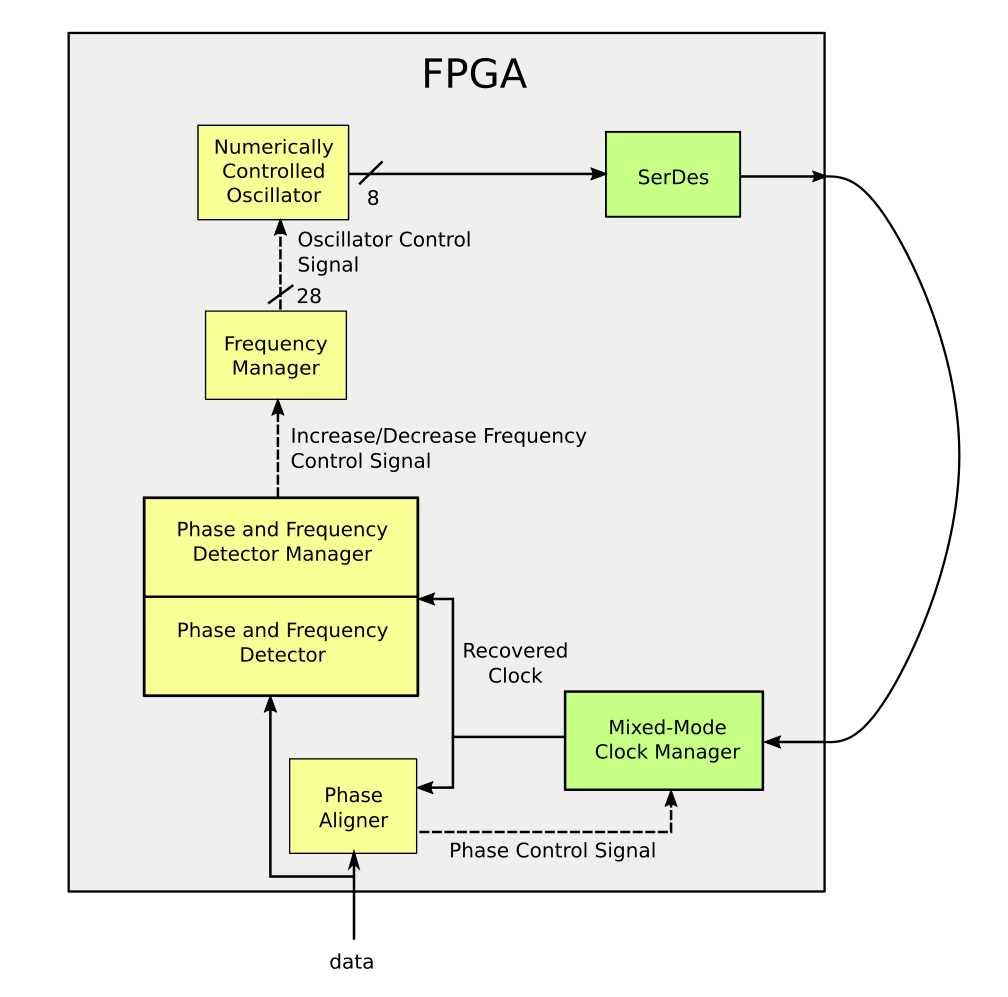
\includegraphics[width=0.5\linewidth]{images/block}}
  \caption{Block diagram for the proposed CDR design. Yellow blocks represents
    custom VHDL modules, green blocks are used to represent FPGA proprietary
    tiles. Dashed lines are used for control signals.}
  \label{fig:cdr_overview}
\end{figure}

The CDR mechanism is similar to the usual PLL architecture, where the phase of a
reference signal is compared to the phase of an adjustable feedback signal,
generally provided by a controlled oscillator, like a Voltage Controlled
Oscillator (VCO). When the phase comparison is in steady state, \textit{i.e.},
the phase and frequency of the reference signal is equal to the phase and
frequency of the feedback signal, we say that the PLL is locked. In the case of
a CDR, the steady state is reached when the VCO clock frequency
matches the reference signal's data rate.\\
The PLL's VCO is substitued in the core's design by a Numerically Controlled
Oscillator (NCO) which is used to create a frequency controlled clock. The
frequency comparator's job is carried out by a Phase and Frequency Detector
(PFD) monitoring the NCO's clock frequency to match it with the data rate, and a
Phase Aligner (PA) that, together with the Xilinx 7 Series MMCME2\_ADV
tile~\cite{ref:mmcm}, dynamically adjusts residual clock drifting and have a
deterministic phase
relationship with the incoming data stream.\\

\subsection{Numerically Controlled Oscillator}
To generate a controlled frequency clock signal, an NCO~\cite{ref:nco} is
employed by the core. Its design consist of two parts:
\begin{itemize}
\item A Phase Accumulator (PACC), which is basically a counter incremented by a
  reference clock.
\item A phase-to-amplitude converter, which uses the PACC output as an index to
  a pseudo-Look-Up Table (LUT)
\end{itemize}
To understand the NCO operation, we can think of a vector rotating around a
phase-circle (Fig.~\ref{fig:phase_wheel}). To each point of this phase-wheel
corresponds a defined value. One revolution of the vector around the
phase-wheel, at costant speed, results in one complete cycle of the output wave.
The PACC counter value corresponds to the points around the phase-wheel, while
the pseudo-LUT assign a specific value to each point. The PACC output value is
increased every system clock cycle, by a specific amount, the \textit{jump size}
(\textit{M} in the picture). The jump size, together with the number of points
in the wheel and the system clock frequency, defines the output wave's
frequency.
\begin{figure}[h]
  \centerline{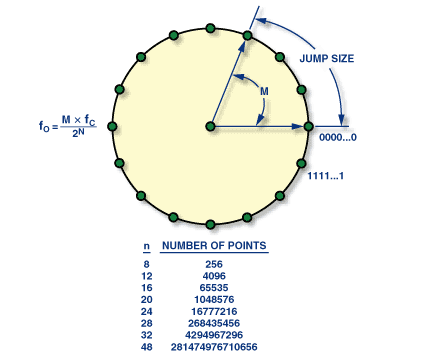
\includegraphics[width=0.4\linewidth]{images/phase_wheel}}
  \caption{The phase-wheel.}
  \label{fig:phase_wheel}
\end{figure}
The correlation between the jump size, the reference clock and the output
waveform frequency is
\begin{equation}
  f_{OUT} = \frac{M \times f_C}{2^N}
  \label{eq:f_out}
\end{equation}
where:
\begin{itemize}
\item $M$ is the jump size
\item $f_{OUT}$ is is the NCO output waveform frequency
\item $f_C$ is the reference clock frequency
\item $N$ is the number of bits dedicated to the PACC counter
\end{itemize}
In order to create a square wave clock signal, the pseudo-LUT assign to half of
the circle the value of '1' while on the other half the value of '0'. This is
done just by taking a specific bit of the PACC counter (hence why the LUT has
been called 'pseudo').\\
However, this desig presents a limitation on the phase resolution: since the
output signal is digital, the time domain is discrete and it corresponds to the
system clock period. This implies the the positive (and negative) fraction of
the output clock signal can only be a multiple of this time domain resolution,
making the output frequency only \textbf{on average} determined by the jump size
of the accumulator. Also, the maximum obtainable output clock frequency
employing this architecture is half of the system clock, which makes it hard to
reach a frequency of 250 MHz, needed for data rates of 250 Mbps.\\
In the next chapter, a way to increase the phase resolution is illustrated. This
will allow the design to work with data rates up to 250 Mbps.\\

\subsubsection{The SerDes Technique} \label{sec:the_serdes_technique} As a first
approach, to improve the phase resolution as well as the output clock frequency,
the system clock shall be increased. This decreases the system clock period
(which equals to the NCO clock phase resolution) and increases the $f_C$
value on Eq.~\ref{eq:f_out}.\\
Even though this approach actually helps to resolve the issues, the reference
clock frequency must comply with the FPGA architecture and can not be increased
over a certain threshold to avoid timing errors.\\
A different approach consist in exploiting the parallelism capability of the
FPGA: instead of just creating one phase-wheel, we generate several of them,
with equal number of points and equal jump size. However, the rotating vector of
these phase-wheels will not compute the same points of the wheel, but they will
span the gap between the phase-points landed by the vector of the first
phase-wheel. After the pseudo-LUT will give value to the phase-points of the
different
wheels, the results are serialized by a SerDes.\\
To clarify, Fig.~\ref{fig:nco_horizontal} presents an example where two
phase-wheels are being generated. For graphical reason, the output will be
represented as a sine waveform instead of a digital 50\% duty cycle clock.\\
The reference clock has a frequency of 250 MHz, therefore every phase-wheel
evaluates a phase-point every 4 ns (Note that the green and blue points are
computed at the same time) and applying Eq.~\ref{eq:f_out}, the resulted
waveform's frequency is 62.5 MHz.\\
To compute the offset in phase-points between each wheel, we refer to the
following equation:
\begin{equation}
  \text{\textit{offset}} = \frac{M}{PW}
  \label{eq:offset}
\end{equation}
where $PW$ is the number of phase-wheels generated and $M$ is the jump size ($PW
= 2, M = 2$ in the example). Note that $M$ must be equal or greater than $PW$.
If the result is fractional, $\text{\textit{offset}}$ is approximated to the
closest integer.
\begin{figure}[h]
  \centerline{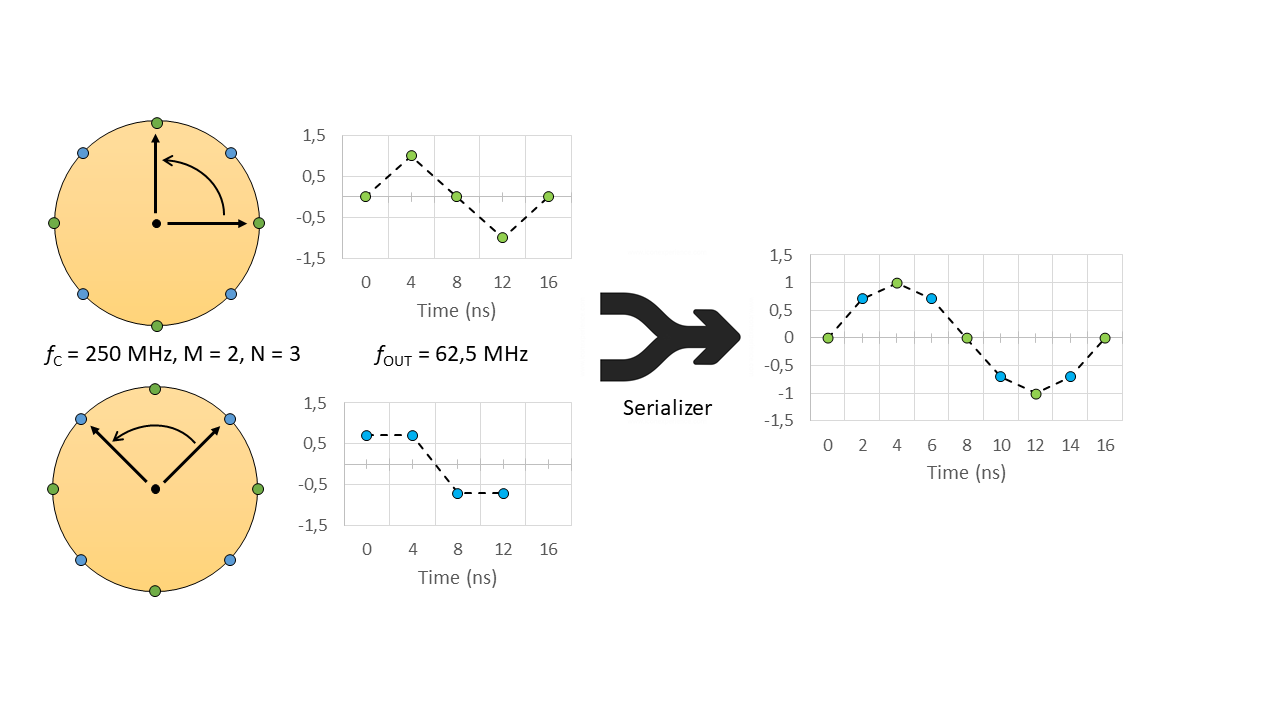
\includegraphics[width=0.9\linewidth]{images/nco_horizontal}}
  \caption{Example of the phase-wheel parallelization technique.}
  \label{fig:nco_horizontal}
\end{figure}
By employing 8 phase-wheels in the CDR core's design with a system clock of 250
MHz, the phase resolution goes from 4 ns to 500 ps. Also, theoretically, the
maximum frequency obtainable by the design is now 2 GHz (of course this is not
possible due to timing errors generation and other issues). By the generic
\textit{g\_multiplication\_factor} the user is able to generate output
frequencies which are higher than the single phase-wheel maximum output
frequency (See Sec.~\ref{sec:generics}). The equation for the overall NCO output
frequency is
\begin{equation}
  f_{OUT} = \frac{M \times f_C}{2^N} * 2^{\text{\textit{g\_multiplication\_factor}} - 1}
  \label{eq:f_out_mult}
\end{equation}
The serialization of the 8 digital bits generated by the pseudo-LUT is carried
out by the OSERDESE2 I/O Kintex 7 tile~\cite{ref:serdes}. Since the OSERDESE2
output must be connected to an I/O Block (IOB) only, a loopback in and out of
the FPGA is a precondition to be foreseen when designing the Printed Circuit
Board (PCB) hosting the FPGA.\\

\subsection{Phase and Frequency Detector}
To match the NCO clock frequency with the data rate, a \textit{Phase and
  Frequency Detector} (PFD)~\cite{ref:cdr} is employed by the core.\\
The PFD frequency detection capability relies on the use of two clock signals,
whose frequency is given by the NCO, with 50\% duty cycle and orthogonal with
each other ($\pi/2$ phase difference). The rising ad falling edges of these two
signals allows the division of the entire 360 degrees of the clock period into
four quadrants, as shown in Fig.~\ref{fig:quadrants}. If the data edges drift up
or down these 4 quadrants, the NCO frequency does not
match the data rate, and needs to be adjusted.\\
The first stage for the data-edges quadrant identification is carried out by the
\textit{Phase Detector Unit} which features a couple of Alexander-type Bang-Bang
phase detectors~\cite{ref:bbpd} connected to the two orthogonal clock waves.
Their outputs consists in early/late pulses (early means that the data has its
edge in the positive half of the clock period, late correspond to the data edge
in the negative half) which are then passed, after a filtering stage based off
an early/late counter, to the \textit{Frequency Detector Unit}. In here two
modules, the \textit{Quadrant Detector} and the \textit{Quadrant Shifting
  Detector} are able to
\begin{itemize}
\item Detect the current quadrant where the data edges resides
\item Store and analyze this information in order to monitor the shifting of the
  data edges quadrant and dictate whether the clock frequency is faster or
  slower than the data rate.
\end{itemize}
When the decision is taken, a \textit{shifting} flag is issued, reporting to the
\textit{Phase and Frequency Detector Manager} in which direction the data edges
are 'climbing' the clock quadrants.
Figure~\ref{fig:PFD},~\ref{fig:PDU},~\ref{fig:FDU} shows the block diagrams of
the VHDL modules.
% \begin{figure}[h]
%   \centerline{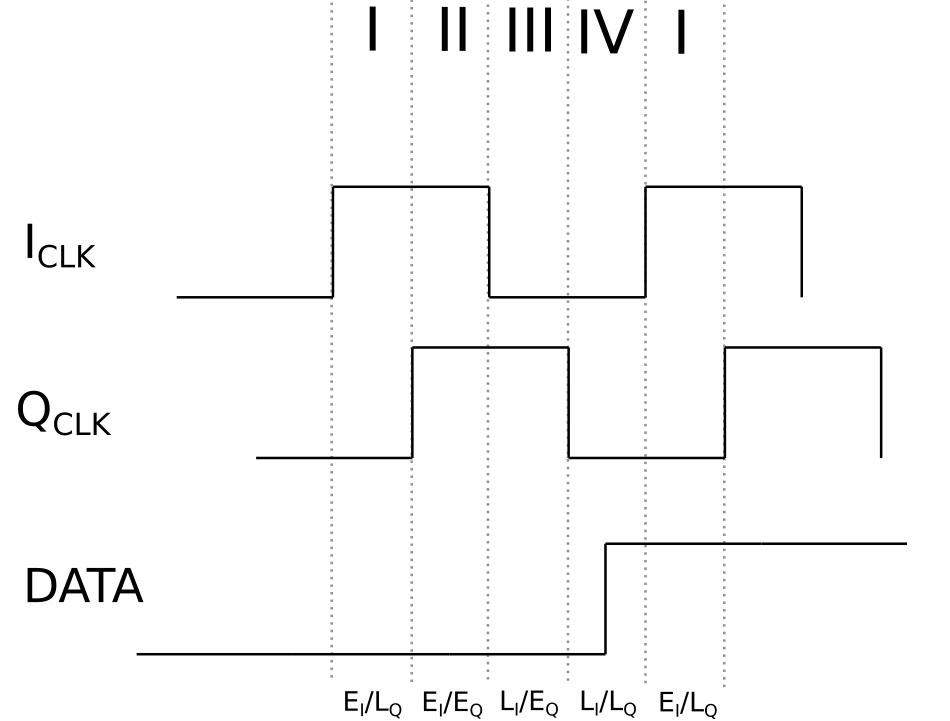
\includegraphics[width=0.4\linewidth]{images/quadrants}}
%   \caption{Two synchronous clocks with 50\% duty cycle, $I_{CLK}$ (In-phase
%   Clock) and $Q_{CLK}$ (Quadrature Clock), divide the period T in four
%   quadrants identified by their positive and negative transitions.
%   $Q_{\textit{CLK}}$ leads $I_{\textit{CLK}}$ by 90 degrees. Thanks to the
%   Early/Late ($E$/$L$) identification by the Phase Detector Unit, it is
%   possible to identify where the \textit{DATA} transitions reside, the fourth
%   quadrant in the example.}
%   \label{fig:quadrants}
% \end{figure}
\begin{figure}[h]
  \centering
  \begin{minipage}[t]{.4\textwidth}
    \centering 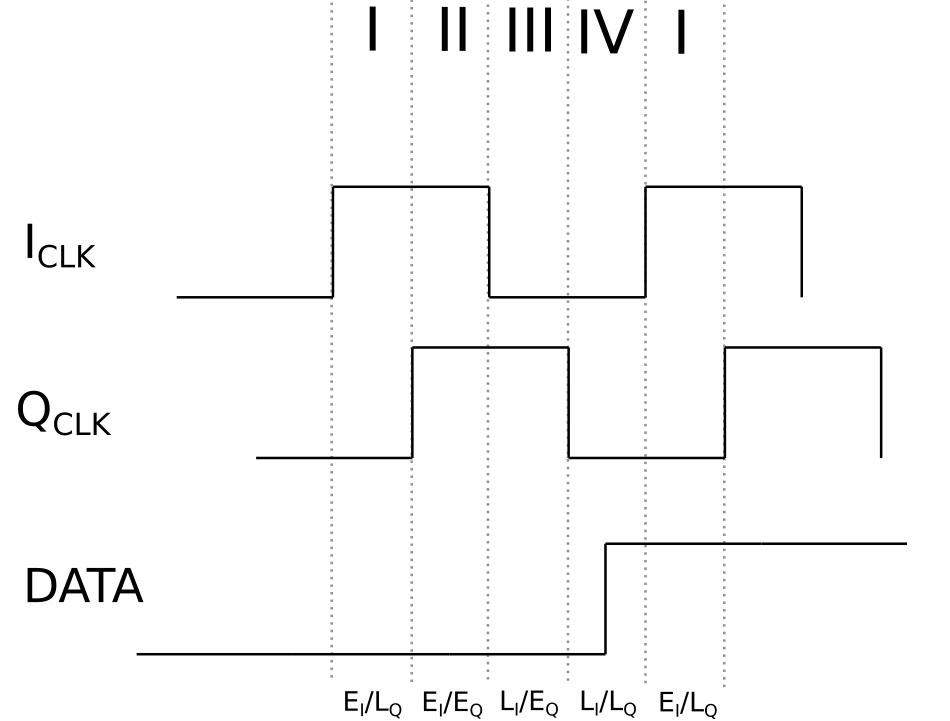
\includegraphics[width=.9\linewidth]{images/quadrants}
    \captionof{figure}{Quadrants definition based on the Early/Late (E/L)
      identification by the Phase Detector Unit. $I_{CLK}$ and $Q_{CLK}$ are two
      synchronous and orthogonal clocks with 50\% duty cycle.}
    \label{fig:quadrants}
  \end{minipage}%
  \hspace{0.5cm}
  \begin{minipage}[t]{.4\textwidth}
    \centering 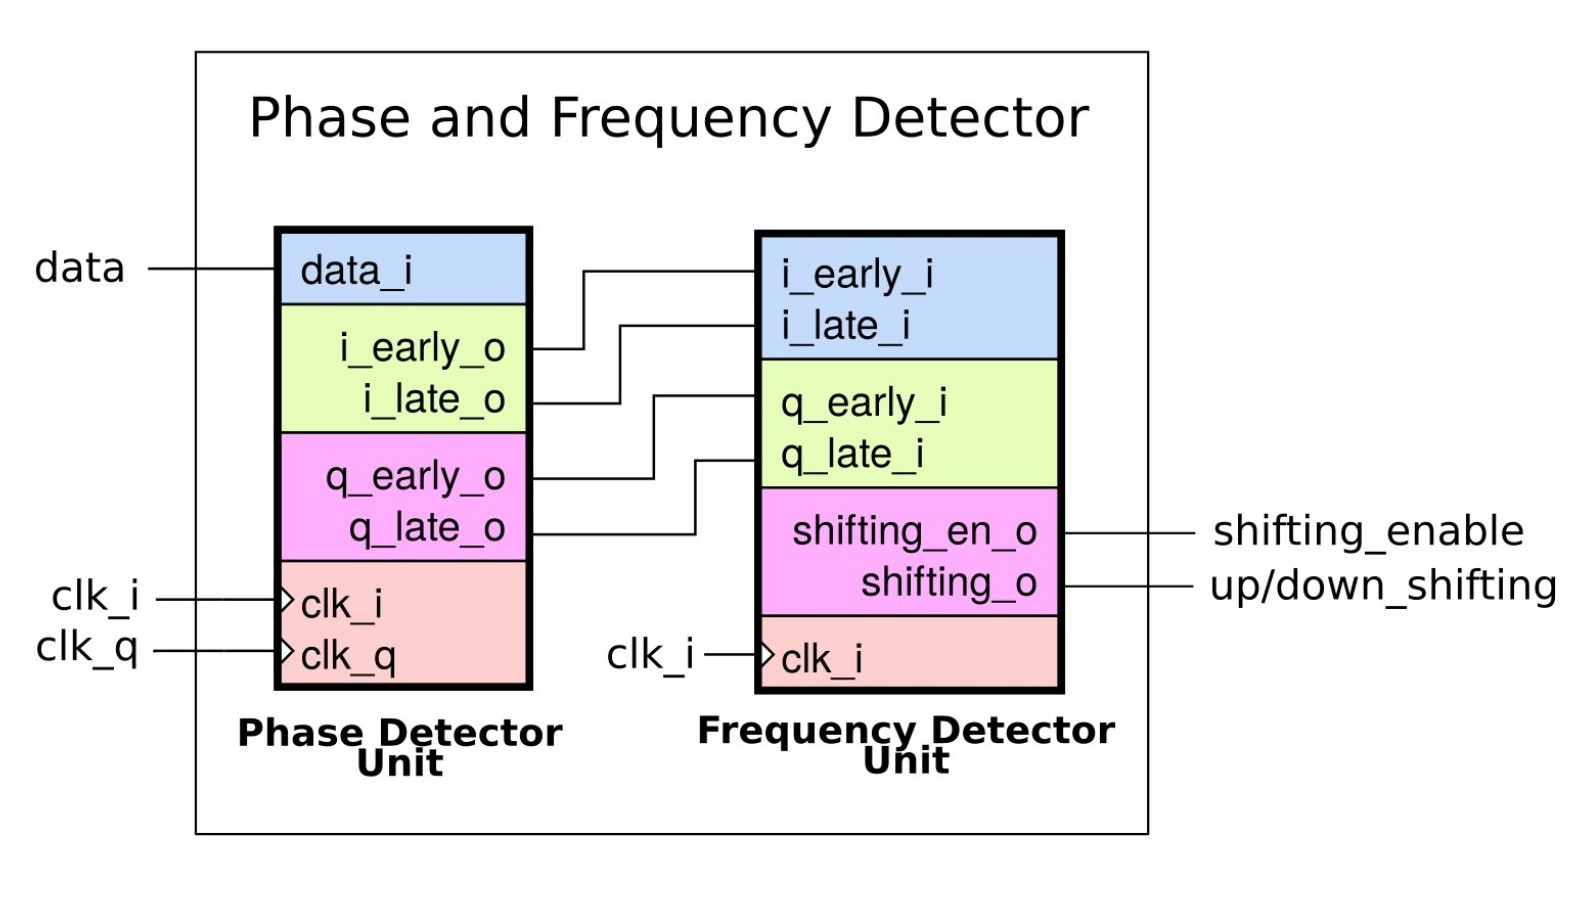
\includegraphics[width=.9\linewidth]{images/blocks/PFD}
    \captionof{figure}{Block diagram of the Phase and Frequency Detector Unit.
      The \textit{shifting\_enable} and \textit{up/down\_shifting} signals
      identify whether the data edge is shifting up (1,1 respectively) or down
      (1,0 respectively) the four quadrants defined by the two clocks in
      quadrature \textit{clk\_i} and \textit{clk\_q}. }
    \label{fig:PFD}
  \end{minipage}
\end{figure}

\begin{figure}[h]
  \centering
  \begin{minipage}[t]{.4\textwidth}
    \centering 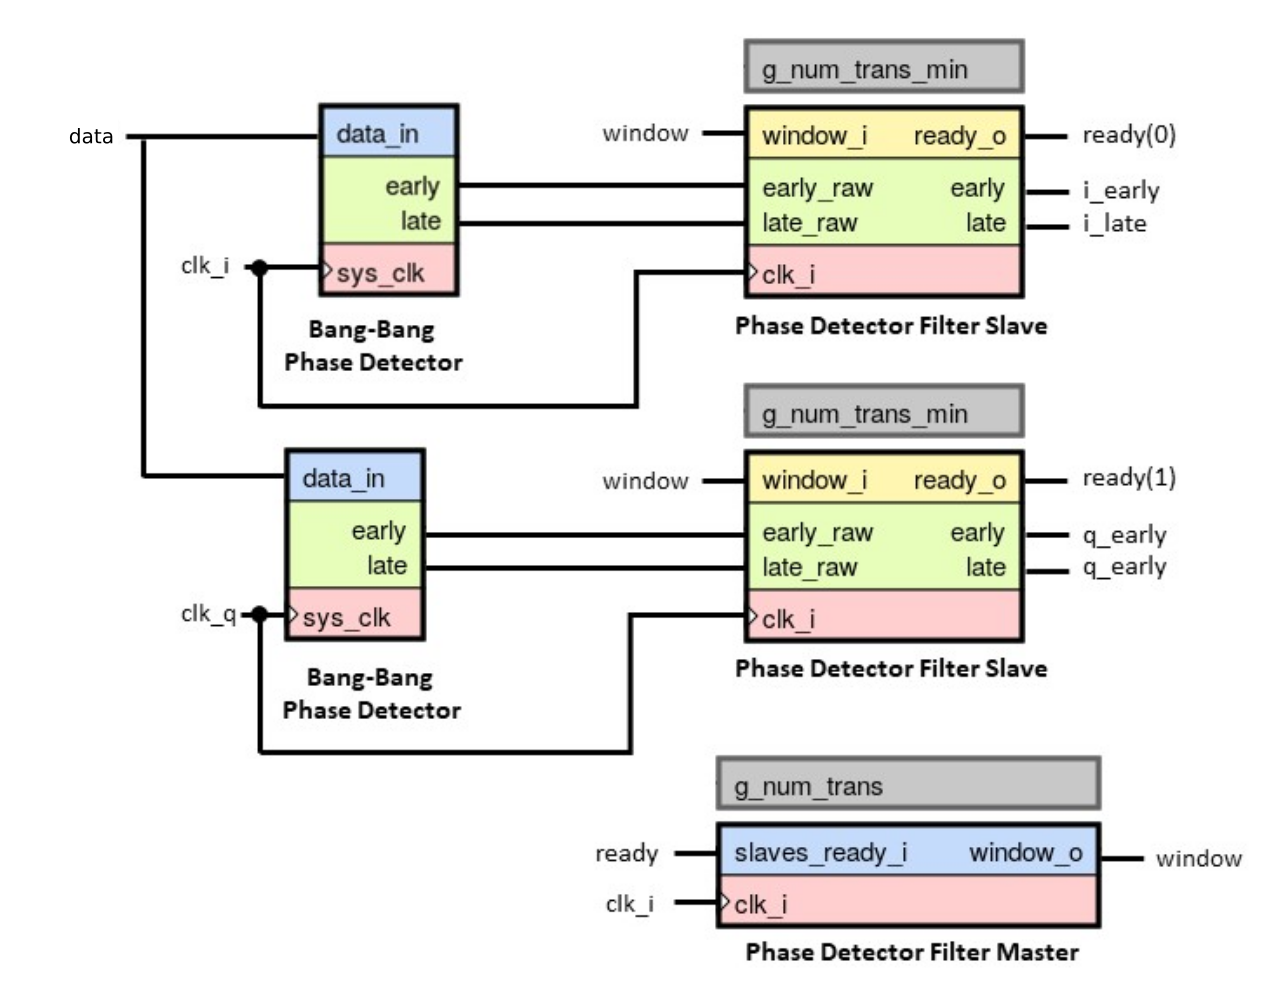
\includegraphics[width=1.0\linewidth]{images/blocks/PDU}
    \captionof{figure}{Block diagram for the Phase Detector unit design. $\cdot$
      the \textit{ready} signals are used by the \textit{Phase Detector Filter
        Master} to start the filtering window $\cdot$ the window length is given
      by $2^{g\_num\_trans}$, while the minimum number of transitions is
      $2^{g\_num\_trans\_min}$}
    \label{fig:PDU}
  \end{minipage}%
  \hspace{0.5cm}
  \begin{minipage}[t]{.4\textwidth}
    \centering 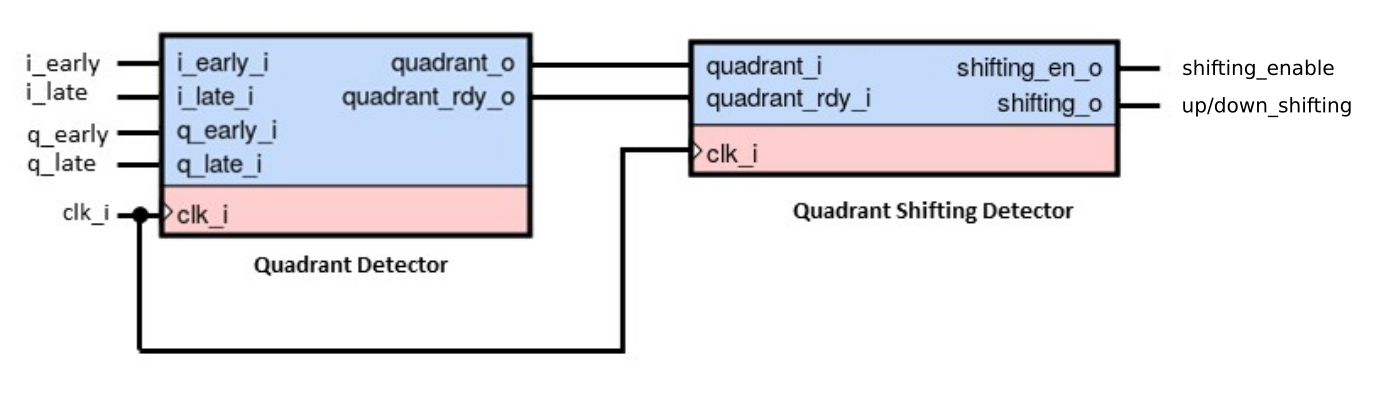
\includegraphics[width=1.0\linewidth]{images/blocks/FDU}
    \captionof{figure}{Block diagram for the Frequency Detector unit design.
      $\cdot$ the \textit{quadrant\_rdy} flag indicates that a new quadrant
      evaluation is ready.}
    \label{fig:FDU}
  \end{minipage}
\end{figure}

\subsection{Phase and Frequency Detector Manager}
Since it is impossible for the clock frequency to perfectly equal the data rate,
due to the finite resolution of the clock frequency and real-world conditions
(\textit{i.e.}, jitter, setup/hold vilations ...), the \textit{Phase and
  Frequency Detector Manager} module exploits a counter method with several
different threshold to get the closest possible frequency as
well as driving the \textit{CDR locked} flag.\\
The counter is set to increase its value when the PFD reports a fester clock
compared to the data, while it decreases on the opposite case. The different
threshold with the related scenarios are:
\begin{itemize}
\item $\pm$ \textit{lock threshold} (around 10\% of the maximum value): inside
  this range the CDR is locked.
\item $\pm$ \textit{activate threshold} (around 50\%): when locked, outside this
  range a frequency change request is forwarded to the NCO.
\item $\pm$ \textit{unlock threshold} (around 90\%): if exceeded, the CDR lock
  flag gets deasserted.
\end{itemize}
Any frequency change request is passed to the \textit{Frequency Manager} module
which adjust the phase-wheel jump size accordingly.\\
When delivering the increase/decrease requests to the \textit{Frequency Manager}
module, the logic signals intersect Clock Domain Crossing (CDC) boundaries. The
PFD design unit is in the NCO's clock domain, while the \textit{Frequency
  Manager}, as well as the NCO itself, are synchronized with the
system clock.\\
To comply with the CDC boundary crossing, a control signal is sent together with
the requests, to avoid erroneous sampling~\cite{ref:cdc}. A timing diagram is
shown in Fig.~\ref{fig:wavedrom}.
\begin{figure}[htbp]
  \centerline{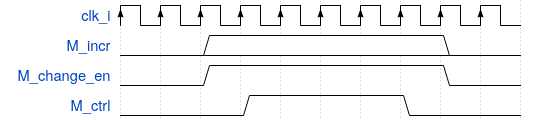
\includegraphics[width=.6\linewidth]{images/wavedrom}}
  \caption{Timing diagram for the PFD frequency shifting requests}
  \label{fig:wavedrom}
\end{figure}

\subsection{Phase Aligner}
The \textit{Phase Aligner} module is needed to eliminate any residual drifting
of the data respect to the clock as well as provide a deterministic phase
relationship, necessary to make sure the sampling is performed in the middle of
the eye pattern, which is the optimal sampling point.\\
Once the PFD is locked, this dynamic phase adjustment is performed by an
Alexander-type Bang-Bang phase detector operating directly on the MMCM,
generating an extra clock signal phase aligned to the data. This is made
possible thanks to the phase shifting capability of Xilinx 7 Series MMCME2\_ADV
tile.

\section{Implementing the Core}
\subsection{Generics} \label{sec:generics} The top-level entity
\textit{top\_cdr\_fpga} has the following generics:
\begin{itemize}
\item \textit{g\_gen\_vio}: if set 'true', the recovered clock frequency is
  settled and fixed by the user through the Xilinx LogiCORE\texttrademark~IP
  Virtual Input/Output (VIO) Core.
\item \textit{g\_check\_jc\_clk}: when 'true', the recovered clock is forwarded
  to its output port through an Output DDR (ODDR) primitive. When 'false', the
  recovered clock dedicated output pin is set to '0'.
\item \textit{g\_check\_pd}: mainly used for debug purposes, this generic gives
  the user the possibility to use two extra ouput pin connected to any top level
  signal, set by the user in the code. If 'false', those output pin are kept at
  '0'.
\item \textit{g\_number\_of\_bits}: positive number setting the length of the
  phase accumulator (a.k.a. number of phase-wheel points), in bits. The total
  number of points will therefore be $2^{\text{\textit{g\_number\_of\_bits}}}$.
\item \textit{g\_multiplication\_factor}: As anticipated in
  Sec.~\ref{sec:the_serdes_technique}, this generic allows the recovered clock
  frequency to be higher than the single phase-wheel maximum obtainable output
  frequency (due to the Nyquist theorem). While the overall recovered clock
  frequency is set by the \textit{g\_freq\_out} generic (see below), the user
  must pay particular attention that
  \begin{equation}\text{\textit{g\_freq\_out}} /
    2^{\text{\textit{g\_multiplication\_factor}} - 1} < \text{\textit{g\_freq\_in}} / 2
  \end{equation}
\item \textit{g\_freq\_in}: system clock nominal frequency in MHz. The system
  clock in the example design is named \textit{s\_clk\_250} and it is generated
  by the \textit{i\_clk\_generator} instance.
\item \textit{g\_freq\_out}: nominal recovered clock frequency in MHz (equal to
  the data rate in Mbps).
\item \textit{g\_out\_phase}: Recovered clock-data phase relationship.
\end{itemize}

\subsection{Ports}
The top-level entity \textit{top\_cdr\_fpga} has the following ports: \bigbreak
Input ports:
\begin{itemize}
\item \textit{sysclk\_p\_i, sysclk\_n\_i}: Differential system clock.
\item \textit{data\_to\_rec\_i}: Incoming data stream to decode through the
  recovered clock.
\item \textit{cdrclk\_p\_i, cdrclk\_n\_i}: Differential NCO output clock from
  the external loopback
\end{itemize}

Output ports:
\begin{itemize}
\item \textit{cdrclk\_p\_o, cdrclk\_n\_o}: Differential NCO output port for the
  external loopback. Output from the SerDes.
\item \textit{cdrclk\_jc\_p\_o, cdrclk\_jc\_n\_o}: If activate from the generic,
  differential recovered clock. Otherwise, the port is tied at '0'.
\item \textit{led\_o}: lock indication from the jitter cleaner MMCM after the
  loopback.
\item \textit{led1\_o}: lock indication from the main MMCM after the loopback.
\item \textit{led2\_o}: lock indication of the CDR core.
\item \textit{led3\_o}: when pulsing, the core is detecting a data stream from
  the \textit{data\_to\_rec\_i} port.
\end{itemize}

\subsection{Core Generation Notes}

\subsubsection{KC705 Example Design Bitstream generation}
The generation of the bitstream for the example design of the core targeting the
KC705 is made through a Tcl script for Xilinx Vivado 2018.3 . Together with the
core, a 'Makefile' is provided. This will automatically generate the VIO core as
well as the complete bitstream. Two options are provided:
\begin{itemize}
\item \textit{make all}: This generates the bitstream without any PRBS error
  checker
\item \textit{make prbs\_check}: run this to generate a Xilinx
  LOGICore\texttrademark~IP Logic integrated Analyzer (ILA) to check te PRBS
  error counter for Bit Error Rate (BER) estimation.
\end{itemize}
Two more FPGA projects are provided: as explained in the test setup dedicated
section (Sec.~\ref{sec:cdr_test}) the example design needs an incoming data
stream. The folders named \textit{dummy\_data\_sender} and
\textit{dummy\_data\_receiver} provide the VHDL code able to generate a PRBS-7
data stream and redirect it to two output ports (Oscilloscope and CDR
implementation board in the tests). Since the boards used for the implementation
are custom, the user may need to adapt the pin constraints file to their choise
of board.

\subsubsection{MMCM's Voltage Controlled Oscillator Frequency}
The two MMCMs encountered by the NCO output clock after the loopback (first one
being the jitter cleaner while the second one being the main phase-controlling
clock manager) must have their internal VCO inside a well defined range,
depending on the FPGA model used. This should be taken into account by the
\textit{freq\_utils} library, whose functions are used to keep the VCO frequency
at 1 GHz, which is well in the range of feasible VCO frequencies for the target
device (Xilinx Kintex-7 XC7K325T-2FFG900C FPGA). The user needs to be careful
when using a different FPGA model that the VCO frequency range complies with the
new chip.

\subsubsection{Changing the 'g\_number\_of\_bits' Generic}
While some applications may find useful to change the 'g\_number\_of\_bits'
generic in order to increase the frequency resolution, some attention should be
placed in doing so. The output frequency needs to be re-calculated using
equation~\ref{eq:f_out_mult}, adjusting the number of bits $N$. The change will
also affect the \textit{frequency\_manager} module as well as the VIO (if used).

\subsubsection{Changing the 'pfd\_manager' Thresholds}
The exact numbers used for the different thresholds set on the
\textit{pfd\_manager} generics instantiation represents the values that returned
the best behaviour from the CDR. It is possible that those numbers are not the
optimal choice when the environment changes (\textit{e.g.}, different data rate,
different data encoding, different physical medium for data transmission ...).\\
The main effect of unwanted behaviour is instability of the 'CDR locked' status.
If this is the observed scenario after implementation, these thresholds may need
to be adjusted.

\section{Simulation}
The CDR core source files comes with several test benches to test the behaviour
of different modules. The simulation files are arranged to be compiled and run
using the GHDL tool~\cite{ref:ghdl} (tested with GHDL v0.37-dev, llvm version)
but are compatible
with any other VHDL simulator (\textit{e.g.}, Vivado simualator).\\
If using GHDL, to compile the simulation run the 'make' command and then run the
executable with GHDL. No automatic tests are predisposed, the user should define
a simulation stop time and dump the wave file.

\subsection{Phase Detector}
The test is useful to understand the behaviour of the Alexander-type Bang-Bang
phase detector by providing a 'random' digital sequence to the module.\bigbreak
Path: \textit{src/hdl/pfd/phase\_detector\_unit/phase\_detector\_tb}

\subsection{Phase and Frequency Detector}
This test bench allows the user to monitor all the modules and sub-modules of
the \textit{phase\_and\_frequency\_detector} entity. This includes the 'Phase
detector unit' and the 'Frequency detector unit'. By providing a data stream
featuring a slightly faster data rate compared to the two input clocks (which
are supposed to derive from the NCO module) the user can observe how the PFD is
able to detect the data rate-clock frequency mismatch and report it.\bigbreak
Path: \textit{src/hdl/pfd/pfd\_tb}

\subsection{Lock Manager}
The first report of a CDR locked status is supplied by the \textit{pfd\_manager}
to the \textit{locker\_manager} module in order to for the final CDR lock status
flag to be delivered.\\
The test bench allows to check the monitoring mechanism of the
\textit{locker\_manager} module. \bigbreak Path:
\textit{src/hdl/lock\_manager\_tb}

\section{CDR Test} \label{sec:cdr_test} As stated in
Sec.~\ref{sec:possible_applications}, the CDR is foreseen to work with data
rates of 125 Mbps. Despite this, the proposed CDR core has the potential to
sustain higher rates, therefore the data rate employed for testing is 250 Mbps,
to which corresponds a recovered clock freqency of 250 MHz (4 ns of clock
period).

\subsection{Test Setup}
\begin{wrapfigure}{l}{0.45\textwidth}
  \begin{center}
    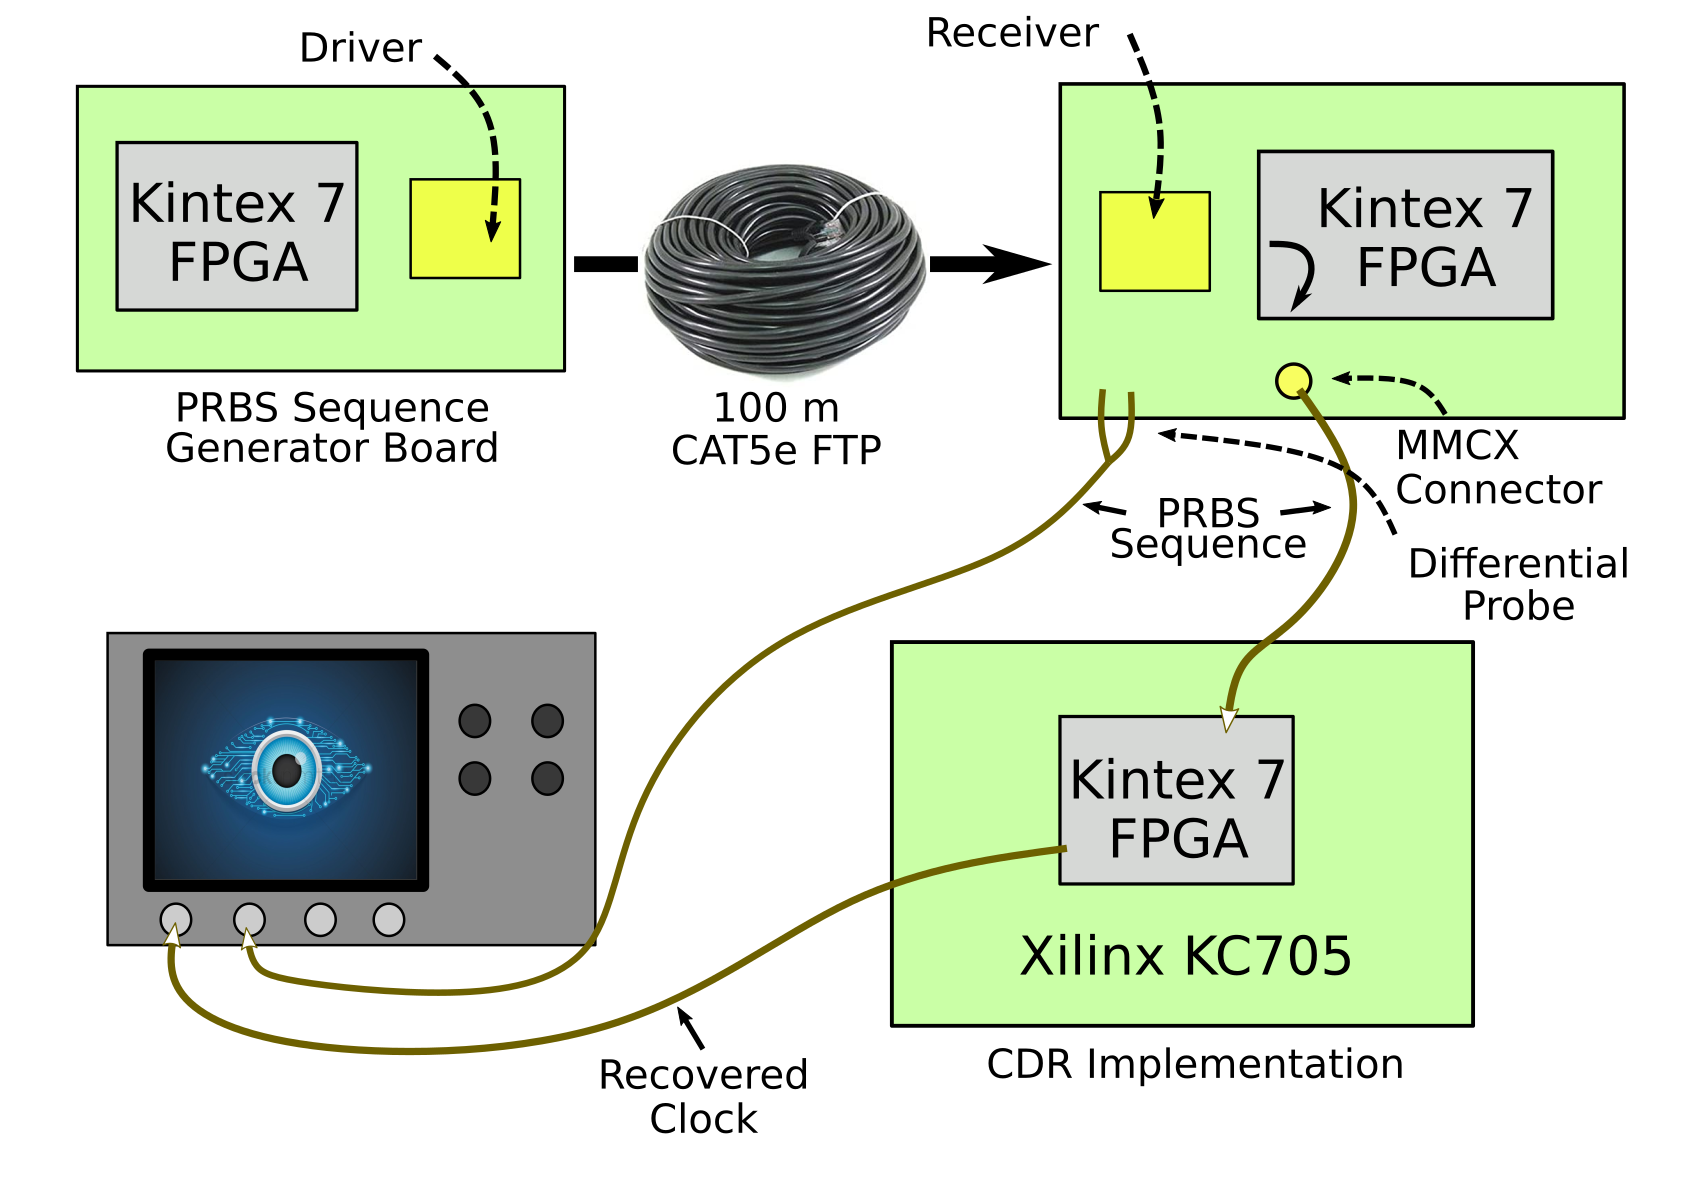
\includegraphics[width=0.9\linewidth]{images/block_setup}
    \caption{Block diagram for the CDR testing setup}
    \label{fig:block_setup}
  \end{center}
\end{wrapfigure}
To test the CDR core performances and capabilities, a PRBS-7 sequence after 100
m of CAT5e Foiled Twisted Pair (FTP) cable is attempted to be recovered. The
data sequence is generated by a JUNO Front-End electronics custom board FPGA, a
Xilinx Kintex-7, and directed to the CAT5e cable after passing through a
differential cable buffer. After 100 m of cable it reaches a second board where
a cable equalizer chip recovers the data sequence. By entering the Xilinx
Kintex-7 FPGA on this second board, the data is forwaded to two output ports: an
MMCX connector connected to the Xilinx KC705 evaluation board hosting the CDR
core and a differential GPIO pin connected to the oscilloscope through a
differential probe. \\
The KC705 exploits the FPGA Mezanine Card (FMC) connector through an FMC
interconnection board to input the PRBS sequence and output the recovered clock,
which is used to trigger the oscilloscope. Together with the CDR core, the KC705
FPGA hosts a PRBS checker module to monitor any error in the recovered
sequence~\cite{ref:prbs}. A block design of the setup is visible in
Fig.~\ref{fig:block_setup}, the physical setup is shown in
Fig.~\ref{fig:setup_v2_numerato}.
\begin{figure}[h]
  \centerline{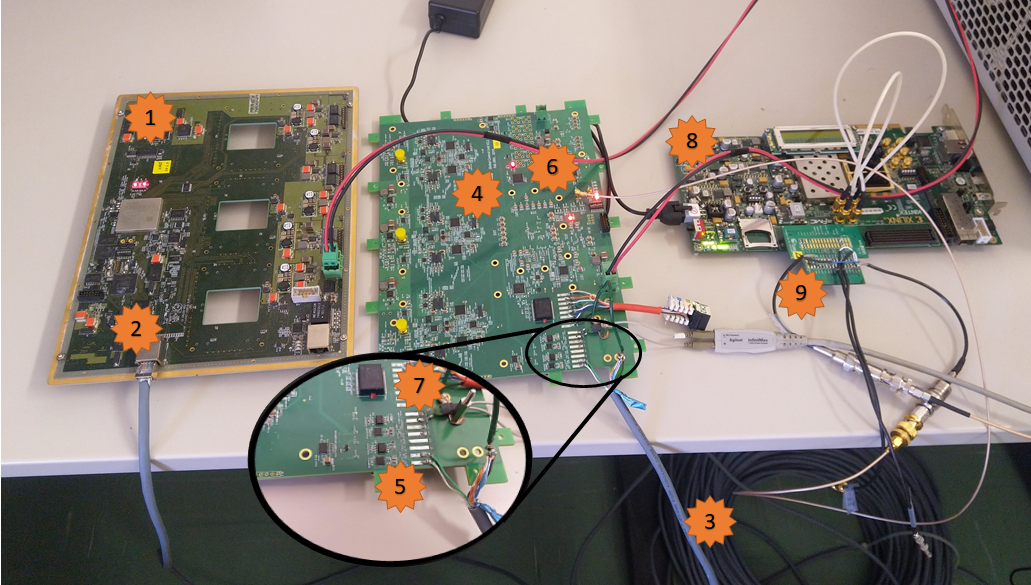
\includegraphics[width=0.7\linewidth]{images/setup_v2_numerato}}
  \caption{Picture of the CDR testing setup. $\cdot$ 1: GCU version 1.0 $\cdot$
    2: RJ45 connector $\cdot$ 3: 100m CAT5e FTP cable $\cdot$ 4: GCU version 2.2
    $\cdot$ 5: RJ45 soldering pads $\cdot$ 6: MMCX connectors $\cdot$ 7:
    Differential probe $\cdot$ 8: Xilinx KC705 evaluation board $\cdot$ 9: FMC
    interconnection board}
  \label{fig:setup_v2_numerato}
\end{figure}

\subsection{Test Results} \label{sec:test_results} The desig is evaluated by
\begin{itemize}
\item Analyzing the eye pattern of the PRBS digital signal after 100m of CAT5e
  cable by triggering the oscilloscope with the CDR recovered clock and setting
  an infinite persistance.
\item Derive the transmission BER monitoring the PRBS error counter module.
\end{itemize}

\subsubsection{Eye Pattern}
The measured eye diagram after the cable transmission is visible on Fig.~\ref{fig:eye}.\\
Thanks to the cable driver buffer and cable equalizer the data is trasmitted and
recovered efficiently, and the vertical opening of the eye has been minimally
impacted by the cable trip. The main issue induced by the cable that could
potentially have an impact on the clock recovery capability of the CDR core, is
jitter. This is visible in the horizontal eye opening of the eye, which is a
combination of data and recovered clock jitter. The width of the eye measured by
the oscilloscope is about 3 ns, guaranteeing a good tolerance for correct data
sampling.

\subsubsection{BER}
To calculate the BER, which is equal to the number of incorrectly received bits
divided by the total number of bits sent, the PRBS error detection capability is
exploited. The KC705 FPGA is equipped, alongside the CDR core, with a PRBS error
counter module, which the user is able to monitor via the Xilinx
LogiCORE\texttrademark~IP ILA.\\
By fixing the BER value at $10^{-12}$ (standard for data transmission over fiber
optics and Ethernet channels) and the CL threshold at 95\%, the reqeuired number
of bits to be decoded without the occurence of any error is about $3 *
10^{12}$~\cite{ref:ber}, corresponding to 200 minutes of error-free data
transmission at 250
Mbps.\\
The test ran for 200 minutes with zero errors counted, allowing to reject the
possibility of a BER higher the $10^{-12}$ with a CL of 95\%.
\begin{figure}[H]
  \centerline{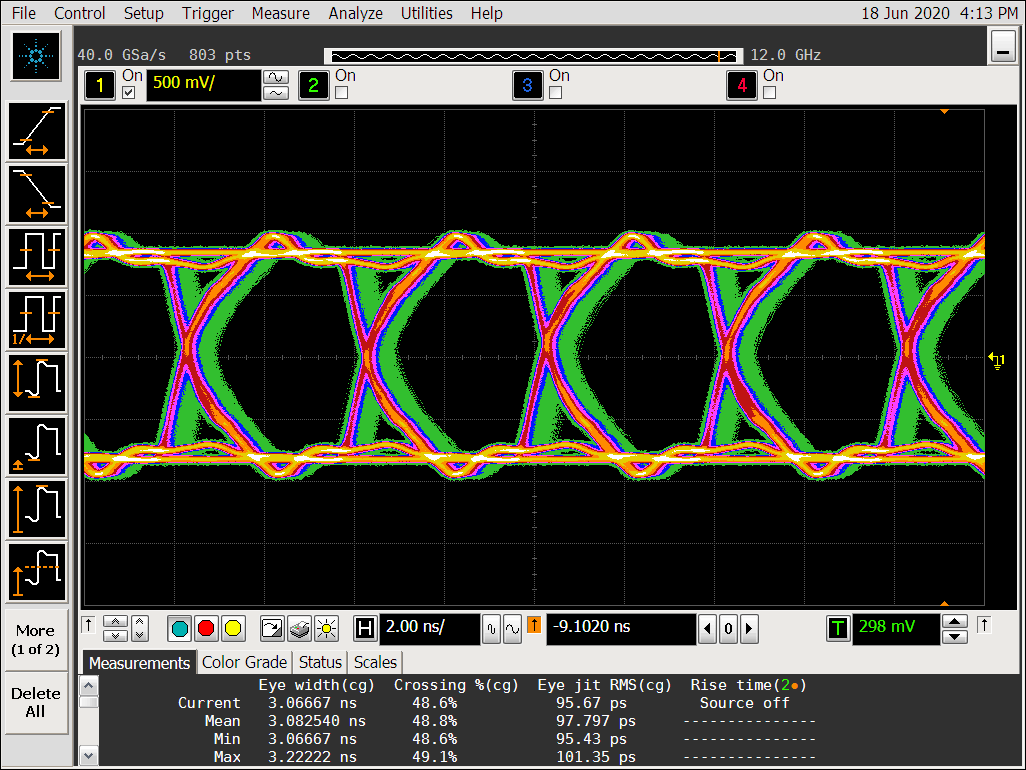
\includegraphics[width=0.6\linewidth]{images/eye_width}}
  \caption{Eye diagram of the PRBS data at 250 Mbps after 100 m of CAT5e cable}
  \label{fig:eye}
\end{figure}

\section{Conclusion}
An FPGA implementation of a fully digital CDR is presented in this report. The
core has been successfully tested against a data rate of 250 Mbps over 100m of
CAT5e FTP cable. The example design accompanying the core targets a Xilinx
Kintex-7 FPGA on a KC705 evaluation board, but it is easily portable to other
FPGAs equipped with a SerDes and a dynamic phase shifting capable clock
management tile.

\begin{thebibliography}{0}
\bibitem{ref:neutrino_physics}F.P. An \textit{et al.}. \textit{Neutrino Physics
    with JUNO}. J. Phys. G43 2016 030401. {\tt arXiv:1507.05613}
\bibitem{ref:juno_cdr}T. Adam \textit{et al.}. \textit{JUNO Conceptual Design
    Report}. {\tt arXiv:1508.07166}
\bibitem{ref:synchronization}D. Pedretti \textit{et al.}. \textit{Nanoseconds
    Timing System Based on IEEE 1588 FPGA Implementation}. IEEE Trans. Nucl.
  Sci. 66 2019 1151. {\tt arXiv:1806.04586v2}
\bibitem{ref:readout_electronics}M. Bellato \textit{et al.}. \textit{Embedded
    Readout Electronics R\&D for the Large PMTs in the JUNO Experiment}. { \tt
    arXiv:2003.08339}
\bibitem{ref:mmcm}Xilinx. \textit{7 Series FPGAs Clocking Resources User Guide
    (UG472)}
  \url{http://www.xilinx.com/support/documentation/user_guides/ug472_7Series_Clocking.pdf}
\bibitem{ref:nco}Eva Murphy and Colm Slattery. \textit{Ask The Application
    Engineer—33: All About Direct Digital Synthesis}. Analog Dialogue vol.38.
  2004.
  \url{https://www.analog.com/en/analog-dialogue/articles/all-about-direct-digital-synthesis.html}
\bibitem{ref:serdes}Xilinx. \textit{7 Series FPGAs SelectIO Resources User Guide
    (UG471)}
  \url{https://www.xilinx.com/support/documentation/user_guides/ug471_7Series_SelectIO.pdf}
\bibitem{ref:cdr}Clock and Data Recovery.
  \url{https://en.wikibooks.org/wiki/Clock_and_Data_Recovery}
\bibitem{ref:bbpd}J.D.H. Alexander. \textit{Clock Recovery from Random Binary
    Signals}. vol. 11. pp. 541 - 542. October 1975 in Electronics Letters.
  Institution of Electrical Engineers.
\bibitem{ref:cdc}Clifford E. Cummings. \textit{Clock Domain Crossing (CDC)
    Design \& Verification Techniques Using SystemVerilog}. SNUG Boston 2008.
  Rev. 1.0
\bibitem{ref:ghdl} \url{http://ghdl.free.fr/}
\bibitem{ref:prbs}Xilinx Application Note, \textit{XAPP884 (v1.0)}. January 10.
  2011.
  \url{https://www.xilinx.com/support/documentation/application_notes/xapp884_PRBS_GeneratorChecker.pdf}
\bibitem{ref:ber}Dragan Mitić, Aleksandar Lebl and Zarko Markov.
  \textit{Calculating the required number of bits in the function of confidence
    level and error probability estimation}. Serbian Journal of Electrical
  Engineering. 9. 361-375. 2012. 10.2298/SJEE1203361M.
\end{thebibliography}



\end{document}
